% 
%  chapter5.tex
%  ISELthesis
%  
%  Created by Matilde Pós-de-Mina Pato on 2012/10/09.
%
\chapter{Implementation}
\label{cha:impl}

This chapter describes how the architecture and resolution cascade introduced in
Chapter~\ref{ch:proposed_solution} are realised in code.

The chapter is organised in three sections. Section~\ref{sec:function-registry} presents the
Function Registry itself: its file format, how entries are created and kept up to date, and the
internal behaviour of the two provider resolvers that consult it at deployment time. The
following section, AWS Lambda Support in QuickFaaS, traces the concrete deployment steps that
Level~3 of the cascade triggers on AWS, work that has no equivalent on the GCP path.
Section~\ref{sec:runtime-invocation} closes the chapter by following a resolved internal call
through to its actual invocation once the workflow has been deployed.

\section{Function Registry}
\label{sec:function-registry}

This work introduces a \textit{Function Registry} to decouple workflow definitions from concrete function endpoints, reducing manual coordination between function deployments and workflow orchestration.

Figure~\ref{fig:omniflow-integration-classes} details the classes that realise the unification inside OmniFlow. Function deployment is abstracted behind the \texttt{InternalFunctionDeployer} interface, following the strategy pattern, with three implementations: \texttt{Noop\allowbreak Internal\allowbreak Function\allowbreak Deployer} (the safe default, which raises if invoked), \texttt{QuickFaasDeployer} (GCP), and \texttt{AwsLambdaDeployer} (AWS). Each provider deployer (\texttt{Google\allowbreak Cloud\allowbreak Deployer}, \texttt{Amazon\allowbreak Cloud\allowbreak Deployer}) owns a provider-specific resolver, and both resolvers share two collaborators: the \texttt{Function\allowbreak Registry\allowbreak Store} and the deployer strategy. The store persists each binding as a \texttt{Function\allowbreak Invocation\allowbreak Metadata} record, in the file format described below. The \texttt{Function\allowbreak Registry\allowbreak Bootstrapper} populates a missing registry by discovery. This structure keeps the two providers symmetric and makes the deployer a clean extension point: supporting a further platform means adding one resolver and one \texttt{InternalFunctionDeployer}, without touching the existing ones.
\begin{figure}[htbp]
  \centering
  
\includegraphics[width=\textwidth]{images/implementation/omniflow-integration-classes.png}
  \caption{Class model of the integration layer added to OmniFlow.}
  \label{fig:omniflow-integration-classes}
\end{figure}


\subsection{Motivation}
A literal \texttt{host}/\texttt{path} ties the workflow definition to one deployment of each
function (Section~\ref{sec:int_cha_int_uni_multi}). The Function Registry removes that tie:
workflows reference internal functions through stable logical identifiers, and the endpoint is
bound to the identifier only at deployment time. Beyond endpoint indirection, the registry also serves as the persistence layer of the
resolution cascade, which creates and refreshes its entries (\S\ref{subsec:registry-updates}).



\subsection{Concept and Conventions}
The DSL-level contract (the \texttt{functionRef} identifier, the
\texttt{internalFunction(name, \allowbreak deployment\allowbreak Descriptor\allowbreak Path)} construct and the rule that
forbids combining it with a literal \texttt{host}/\texttt{path}) is defined in
\S\ref{sec:dsl-extensions}, with an example call step in Listing~\ref{lst:call-step-internal}.
What matters for the implementation is where that rule is enforced: the DSL builder rejects
the illegal combination when the workflow is constructed, and each resolver checks it again before
rendering, so an ambiguous call can never reach a provider artifact.

\subsection{Registry File Format}
The file format is the one described in \S\ref{sec:dsl-extensions} and shown in
Listing~\ref{lst:registry-structure}: one JSON file per provider
(\texttt{function-registry.gcp.json} or \texttt{function-registry.aws.json} by default), holding
only non-secret invocation metadata. Two conventions become visible only in a registry that has been in use. A function deployed by QuickFaaS on GCP is stored under its plain \texttt{functionRef}, with a first-generation \texttt{cloudfunctions.net} URL; a Cloud Run service found by discovery is stored under a region-qualified key such as \texttt{"europe-west1/risk-score"}, whose \texttt{serviceName} is the full resource name \texttt{projects/proj/locations/europe-west1/services/risk-score} rather than the bare service id. The file is kept in a writable location (the working directory by default, or a path given to the deployer), never inside packaged resources, which are typically read-only in production.

\subsection{Creation, Bootstrap and Updates}
\label{subsec:registry-updates}
The registry management layer provides the following behavior:

\begin{itemize}
    \item \textbf{Bootstrap by discovery:} if the registry file does not exist when a workflow with
    internal calls is deployed, it is created automatically by listing the functions already
    deployed on the target provider (Cloud Run services on GCP, Lambda functions on AWS) and
    writing one entry per discovered function; on
    AWS this scans every region enabled for the account and, mirroring the GCP catalog, promotes a
    function name seen in more than one region from a bare key to a \texttt{"region/name"} key for
    each occurrence.
    \item \textbf{Automatic registration:} when an internal function is not present in the
    registry but is found on the target provider (Cloud Run service on GCP, Lambda function
    on AWS), a new entry is written immediately with the discovered metadata.
    \item \textbf{Post-deployment updates:} after a successful QuickFaaS deployment, the
    resulting invocation metadata is written to the registry, so subsequent deployments
    resolve the function without redeploying it.
    \item \textbf{Drift handling:} on every registry hit, the stored endpoint is validated
    against the live resource (Cloud Run service on GCP, Lambda function on AWS) and the entry is
    refreshed if it changed; a resource that no longer exists is treated as a stale entry
    (\S\ref{sec:walkthrough}), except for first-generation Cloud Functions on GCP
    (\S\ref{subsec:store-internals}).
\end{itemize}

Every write refreshes the top-level \texttt{updatedAt} timestamp.

\subsection{Deployment-Time Endpoint Resolution}
\label{subsec:endpoint-resolution}
The registry is consumed at deployment time by an endpoint resolution step that runs before the
provider-specific artifact (e.g., Google Workflows YAML) is rendered. OmniFlow traverses the
workflow tree (including nested branches, iterations and parallel blocks) and intercepts
every \texttt{CallContext} carrying an \texttt{internalFunction} declaration, leaving external
calls untouched. Each intercepted call is then put through the three-level cascade defined in
\S\ref{sec:resolution-cascade}: a registry hit validated against the live resource, provider
discovery across regions, and a QuickFaaS deployment as a last resort. The levels are not restated
here; \S\ref{subsec:store-internals} describes how the two resolvers realise them, and
\S\ref{subsec:validation-error-semantics} the errors they raise when a call cannot be bound.

The resolved URL is finally split into \texttt{host} and \texttt{path} (on AWS, into a
\texttt{lambda://<arn>} reference consumed by the renderer) and injected into the call step
before the provider-specific workflow artifact is rendered.
\subsection{Registry Store and Resolver Internals}
\label{subsec:store-internals}

The registry file is manipulated exclusively through \texttt{FunctionRegistryStore}, which
exposes a small, deliberately narrow interface: \texttt{readAll()} parses the whole file into an
ordered map of \texttt{functionRef} to \texttt{FunctionInvocationMetadata}; \texttt{tryResolveEntry()}
re-reads the file via \texttt{readAll()} and delegates the two-step lookup (exact match on
\texttt{functionRef}, then suffix match on \texttt{"region/\allowbreak functionRef"}, raising if the suffix
match is ambiguous) entirely to its pure counterpart, \texttt{tryResolveEntryIn()}, which performs
that lookup against an already-loaded map with no I/O of its own (the same split
\texttt{resolveUrl()}/\texttt{resolveUrlIn()} already had); \texttt{put()} inserts or refreshes one entry; and
\texttt{remove()} deletes a stale entry. The store itself keeps no in-memory state between calls, so
\texttt{readAll()}/\texttt{tryResolveEntry()} re-read and re-parse the file on every call; the
performance consequences of this choice are analysed in Chapter~\ref{cha:evaluation}.

The two provider resolvers sit on top of this store. \\
\texttt{WorkflowInternalFunctionResolver} (GCP) treats a registry hit as provisional: it
validates the stored URL against the live Cloud Run service and, if the URL has drifted, refreshes
the entry; if the service has disappeared, it attempts rediscovery across the project's regions
and, failing that, removes the stale entry and aborts. It also short-circuits validation for
first-generation Cloud Functions (identified by a \texttt{cloudfunctions.net} URL), which are not
Cloud Run services. When a function is absent from the registry, it is looked up across regions,
and a match in more than one region is reported as ambiguous.\\
\texttt{Aws\allowbreak Internal\allowbreak Function\allowbreak Resolver} follows the same shape: it treats a registry hit
as provisional, resolving the region to validate from the stored ARN and consulting the Lambda API
through a \texttt{Lambda\allowbreak Function\allowbreak Inspector} seam; a drifted ARN refreshes the entry, and a
permissions failure aborts rather than being mistaken for an absence. The resolver mirrors the GCP path and attempts
rediscovery, searching every region enabled for the account before removing the stale entry and
aborting. \\
Region discovery is itself provider-specific: GCP already exposed a project-scoped
locations API, whereas AWS has no equivalent for Lambda, so a dedicated
\texttt{Ec2Aws\allowbreak Regions\allowbreak Lister}, backed by the EC2 \texttt{DescribeRegions} call, was added to
play that role; an optional preferred region, when supplied, is tried first in both the
rediscovery and the miss-path scan described next. \\
On a registry miss, the AWS resolver performs
the same style of scan as GCP: it searches every enabled region for a function-name match and
reports a name found in more than one region as ambiguous; the caller skips the scan by supplying
the fully-qualified \texttt{"region/functionRef"} form, which resolves a single region directly. Regions where the
lookup is refused are handled as on the GCP path (\S\ref{subsec:validation-error-semantics}). What
distinguishes the two resolvers is only the underlying provider API each one calls (the Cloud
Run Locations API versus EC2 \texttt{DescribeRegions} for region discovery, a Cloud Run lookup
versus \texttt{GetFunction} for the per-region check) and the GCP-only short-circuit noted above.
In both resolvers, a successful
discovery or deployment writes the metadata back through \texttt{put()} before the endpoint is
injected into the call, and so does a hit whose endpoint has drifted (a hit that validates
unchanged writes nothing), so the registry converges toward a complete set of bindings as workflows
are deployed.

To keep resolution cheap when a workflow contains many internal calls, both provider resolvers
read the registry once into a snapshot at the start of \texttt{resolve()} and resolve every call
against that in-memory map, keeping it in sync with every subsequent \texttt{put()}/\texttt{remove()}
so that two calls to the same function within one workflow still observe each other's writes,
rather than re-reading the file per call.

\paragraph{Limitation: first-generation Cloud Functions on GCP.}
On GCP, QuickFaaS deploys first-generation Cloud Functions (\S\ref{sec:background_quickfaas}),
but the GCP resolver's live validation, its provider discovery and the registry bootstrap all query
the Cloud Run API. The functions that the integration itself deploys on GCP are therefore only
partly covered by the cascade. First, a registry hit on a \texttt{cloudfunctions.net} URL is
returned without a live check, so a function that was deleted or moved is not detected at
deployment time: the workflow is deployed against the stored URL, and the failure only surfaces
when the workflow invokes the function. Second, neither the bootstrap nor discovery lists
first-generation functions, so a binding missing from the registry (for example, because the
registry file was deleted or the deployment runs on another machine) cannot be rediscovered. With a
descriptor, the cascade reaches Level~3 and invokes QuickFaaS again for a function that already
exists; without one, deployment fails and reports the function as absent. The AWS path is not
affected. Closing the gap requires QuickFaaS to deploy through the Cloud Functions~v2 API, so that
the functions it creates are Cloud Run services and fall under the validation, discovery and
bootstrap already implemented; this is listed as future work (Section~\ref{sec:concl-future}).

\subsection{Resolution Cascade Sequences}
\label{subsec:cascade-sequences}

The description of the two resolvers above is expanded into six sequence diagrams, one per
cascade level and provider, making explicit the messages exchanged with the registry and with
each provider's inspection API; to keep this chapter's flow uninterrupted, the diagrams themselves
are collected in Appendix~\ref{app:cascade-sequences} rather than placed inline:
Figure~\ref{fig:resolution-cascade-level1} for Level~1,
Figure~\ref{fig:resolution-cascade-level2} for Level~2 and
Figure~\ref{fig:resolution-cascade-level3} for Level~3, each contrasting the GCP panel (a) with
the AWS panel (b) and captioned with the behaviour it shows.

The Level~3 panels stay at the cascade's conceptual level; the operational steps of the AWS
branch are traced for the worst-case path in Figure~\ref{fig:aws-deploy-sequence}, introduced in
the AWS Lambda Support section that follows.

\subsection{Validation and Error Semantics}
\label{subsec:validation-error-semantics}
Several correctness constraints are enforced to avoid silent misconfiguration. Three of them, an
unresolvable function, an ambiguous reference and a stale registry entry, are stated with the rest
of the cascade's failure modes in \S\ref{sec:walkthrough}, and all abort the deployment before any provider artifact is
rendered. One consequence of the second belongs here: an ambiguous reference is not rescued by
supplying a \texttt{deploymentDescriptorPath}, because ambiguity is a data-consistency problem
rather than an absence one, so QuickFaaS is never invoked to paper over it. The remaining
constraint is implementation-level.

\paragraph{Insufficient permissions.}
If the live lookup used to validate a registry hit is refused (an authorization failure rather
than an absence), deployment aborts immediately with a diagnostic naming the function; on GCP no
rediscovery is attempted, since a permissions failure gives no information about whether the
service still exists. The same rule applies on AWS, where a refused \texttt{GetFunction} is
likewise distinguished from a genuine absence. The distinction is drawn more coarsely on the
miss-path region scan, on both providers: while the scan is running, a region where the lookup is
refused is simply excluded from the candidate set, the same as a region where the function is
absent, so a permissions gap in one region does not by itself stop a match found elsewhere; but if
the scan ends with no match anywhere and at least one region could not be checked, it surfaces a
diagnostic naming the inaccessible regions instead of silently concluding the function is absent
everywhere.

\subsection{Evolution of the Registry Design}
\label{subsec:registry-evolution}

The registry did not arrive at its current form in a single step; the source tree still exposes
the intermediate stages, which makes the design decisions worth recounting. Its starting point was
the indirection motivated above; four threads describe how it evolved from there.

\paragraph{A metadata record per function.}
Each function is represented in the registry by a single structured record,
\texttt{FunctionInvocationMetadata}, which the two
production resolvers, \texttt{Aws\allowbreak Internal\allowbreak Function\allowbreak Resolver} and
\texttt{Workflow\allowbreak Internal\allowbreak Function\allowbreak Resolver}, consume directly (\S\ref{subsec:store-internals}), at the cost
measured in Section~\ref{sec:eval-real-resolvers}. The same single-read strategy, isolated from any
cloud-side validation, is also implemented by a benchmark fixture,
\texttt{OptimizedEndpointResolver}, which the local-resolution benchmark suite uses as a pure,
provider-agnostic reference implementation, deliberately decoupled from the live-validation step
the real resolvers must perform against a cloud API.

\paragraph{From provider-specific fields to a uniform endpoint.}
Collapsing the endpoint into one \texttt{url} field was the change that made the AWS extension
cheap. Because \texttt{url} is treated as an opaque, provider-interpreted string (an HTTPS
endpoint on GCP, a Lambda ARN on AWS), the registry schema did not have to change when the AWS
provider was added; only the resolver that reads the field and the renderer that consumes it are
provider-aware. The registry thus stayed a single, symmetric abstraction across the two clouds.

\paragraph{From a manually edited file to an auto-managed source of truth.}
The registry also evolved from something the developer would maintain by hand into something the
integration maintains automatically, through the bootstrap, registration, refresh and pruning
listed in \S\ref{subsec:registry-updates}. In parallel, the resolution path itself was refined from
re-reading the whole file on every lookup (\texttt{resolveUrl}) toward reading it once into a
snapshot and resolving in memory (\texttt{readAll} + \texttt{resolveUrlIn}); the performance effect
of that refinement, and its propagation into the two production resolvers, are quantified in
Chapter~\ref{cha:evaluation}.

\paragraph{From a trusted cache to a verified indirection.}
The two production resolvers did not always treat a registry hit the same way.
\texttt{Workflow\allowbreak Internal\allowbreak Function\allowbreak Resolver} (GCP) validated every hit against the live
Cloud Run service from the start, because a Cloud Run lookup needs the project/region/service
triple that only the registry supplies. \texttt{Aws\allowbreak Internal\allowbreak Function\allowbreak Resolver} initially
trusted a hit outright, returning the cached ARN with no live check, since a Lambda name is
already unique within a region and validating brought no discovery benefit on its own. This
asymmetry was closed by introducing \texttt{Lambda\allowbreak Function\allowbreak Inspector}, the AWS counterpart to
the Cloud Run inspector: a hit is now confirmed against \texttt{GetFunction} on both providers,
refreshing a drifted ARN and removing a deleted one. The change did not make the registry
redundant, only its trust model stricter: the live check answers whether a binding the registry
already named is still accurate, not what to look up or whether a deployment is owed. Indirection
and idempotency, the two properties that motivated the registry in the first place
(\S\ref{sec:resolution-cascade}), are unaffected by whether the hit is trusted or verified.

\section{AWS Lambda Support in QuickFaaS}
Figure~\ref{fig:aws-deploy-sequence} traces the end-to-end deployment on AWS, from the registry bootstrap to \texttt{Create\allowbreak State\allowbreak Machine}, and expands the most demanding path, where an internal function exists in neither the registry nor AWS. The \texttt{alt} fragment has one branch for each of the three levels of the resolution cascade described in Section~\ref{subsec:endpoint-resolution}, and a fourth for the calls that fail fast. Once Level~3 is reached, \texttt{AwsLambdaDeployer} performs the AWS-specific work described step by step in Section~\ref{subsec:omniflow-aws-deployer}. The ARN it returns is stored in the registry and, once all calls are resolved, the workflow is rendered with a \texttt{lambda:invoke} task resource and submitted via \texttt{Create\allowbreak State\allowbreak Machine}. This diagram makes explicit the operational steps that the conceptual cascade abstracts away. The rationale for invoking QuickFaaS as a subprocess, rather than integrating the two tools as separate communicating services, is discussed in Section~\ref{sec:design-rationale}.

\begin{figure}[htbp]
  \centering
  
\includegraphics[width=\textwidth]{images/implementation/aws-deploy-sequence.png}
  \caption{Deployment sequence on AWS, with one branch per level of the resolution cascade and
  the Level~3 path (function absent from both the registry and the provider) expanded.}
  \label{fig:aws-deploy-sequence}
\end{figure}

AWS support is realised in two layers that meet at the subprocess boundary: the AWS provider added
\emph{inside} QuickFaaS, which performs the actual Lambda deployment, and the
\texttt{Aws\allowbreak Lambda\allowbreak Deployer} added \emph{inside} OmniFlow, which prepares the environment,
drives QuickFaaS, and produces the invocation metadata the registry stores.

\subsection{The QuickFaaS AWS Provider}
\label{subsec:quickfaas-aws-provider}

The AWS provider extends QuickFaaS's existing abstractions (\texttt{CloudProvider},
\texttt{Cloud\allowbreak Function}, \texttt{CloudRequests}) so that a cloud-agnostic function can be packaged
and deployed to AWS Lambda through the same ZIP strategy used for GCP and Azure. Its core is
\texttt{AwsLambdaFunction.deployZip}, which: uploads the packaged archive to the S3 bucket named in
the descriptor; checks whether the function already exists (\texttt{GetFunction}); and then either
creates it (\texttt{CreateFunction}, with the code referenced as an S3 object) or updates its code
(\texttt{UpdateFunctionCode}), in both cases blocking on the AWS SDK waiter until the function is
active. The handler is fixed to the provider-agnostic entry point \texttt{AwsHttpTemplate}, which
adapts the Lambda request to the developer's hook, and the supported runtimes are \texttt{java11}
and \texttt{java17}. Because \texttt{GetBucketLocation} must be issued against the global endpoint,
the provider resolves the bucket's region from \texttt{us-east-1} and then pins the Lambda client
to that same region, ensuring the function and its code bucket are co-located. Finally, the
provider creates (or reuses) a Lambda \emph{Function URL} with \texttt{AuthType = AWS\_IAM},
QuickFaaS's own notion of an invocation endpoint, which the OmniFlow integration does not use.

\subsection{The OmniFlow-Side Deployer}
\label{subsec:omniflow-aws-deployer}

\texttt{AwsLambdaDeployer} is the AWS implementation of the \texttt{InternalFunctionDeployer}
strategy. It performs the work that has no GCP equivalent and that must happen \emph{around} the
QuickFaaS subprocess. From the raw descriptor it resolves or creates the Lambda execution IAM role:
if \texttt{iamRoleArn} is blank or a placeholder, it creates a managed
\texttt{OmniFlowLambdaExecutionRole} (attaching \texttt{AWSLambdaBasicExecutionRole}); if a real ARN
is supplied, it verifies and, if necessary, repairs the role's trust policy so that
\texttt{lambda.amazonaws.com} can assume it. The resolved ARN is patched into a temporary copy of
the descriptor, the effective region is taken from the S3 bucket's location, and QuickFaaS is
invoked as a subprocess, retried up to three times with a 20-second back-off to absorb IAM
eventual consistency. After the subprocess returns, the deployer polls \texttt{GetFunction} until
the function reports the \texttt{Active} state (bounded by a 180-second timeout), retrieves the ARN,
and grants the Step Functions service principal permission to invoke the function.

A deliberate design choice is visible here: although the QuickFaaS provider produces a Function URL,
the OmniFlow deployer discards it and stores the \emph{ARN} in the registry, because internal calls
are rendered with the native \texttt{lambda:invoke} integration (Section~\ref{sec:runtime-invocation})
rather than as HTTP calls to a Function URL. Listing~\ref{lst:aws-descriptor} shows a minimal AWS
deployment descriptor: it differs from the GCP descriptor of
Listing~\ref{lst:quickfaas_json_config} mainly in \texttt{cloudProvider}, the S3 \texttt{bucket},
the Lambda \texttt{runtime}, and the \texttt{iamRoleArn} field (which may be left as a placeholder to
request automatic role creation).

\begin{lstlisting}[language=json,caption={Minimal AWS deployment descriptor for an internal function.},label={lst:aws-descriptor}]
{
  "cloudProvider": "aws",
  "project": "123456789012",
  "iamRoleArn": "<auto>",
  "function": {
    "name": "hello-lambda-fn",
    "location": "eu-west-1",
    "bucket": "run-sources-tfm2526-eu-west-1",
    "runtime": "java17",
    "trigger": { "type": "http" }
  },
  "functionFile": "./MyFunctionClass.java"
}
\end{lstlisting}

\section{Runtime Invocation}
\label{sec:runtime-invocation}
Figure~\ref{fig:aws-runtime-invocation} shows how an internal function is invoked at runtime, once the workflow is deployed. Step Functions invokes the Lambda directly, through the native \texttt{arn:aws:states:::lambda:invoke} integration and with the ARN fixed at deployment time, passing it the step's payload; the QuickFaaS template entry point adapts the request and delegates to the developer's hook function, and the response is returned under \texttt{\$.Payload}. Using the native integration rather than an HTTP endpoint avoids per-call request signing and keeps the invocation within the AWS control plane.

\begin{figure}[htbp]
  \centering
  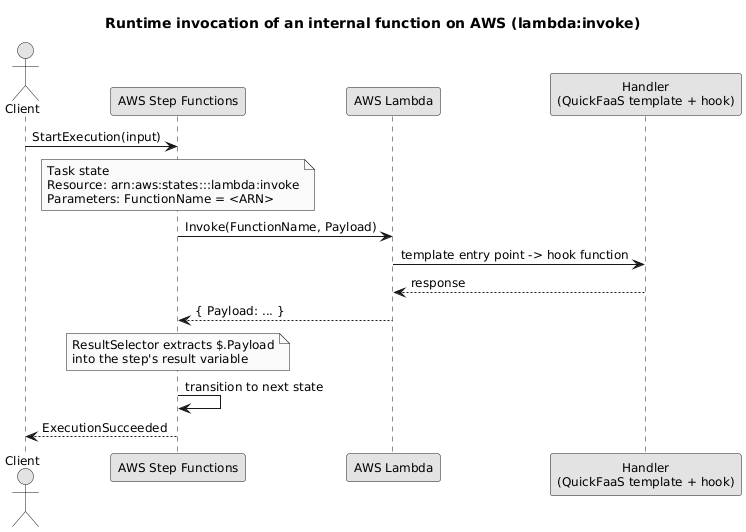
\includegraphics[width=0.8\textwidth]{images/implementation/aws-runtime-invocation.png}
  \caption{Runtime invocation of an internal function on AWS via the native
  \texttt{lambda:invoke} integration.}
  \label{fig:aws-runtime-invocation}
\end{figure}


Internal and external calls are told apart entirely by the renderer,
\texttt{AmazonCall\allowbreak Renderer} (whose emitted resource strings live in
\texttt{AmazonConstantsUtils}), from the \texttt{host} value injected during resolution. If the host
carries the \texttt{lambda://} prefix (the marker written by \texttt{Aws\allowbreak Internal\allowbreak Function\allowbreak Resolver}),
the renderer emits a \texttt{Task} whose \texttt{Resource} is
\texttt{arn:aws:states:::lambda:invoke} and whose \texttt{Parameters} carry the
\texttt{FunctionName} taken from the resolved ARN; any query terms are forwarded under a
\texttt{Payload.queryStringParameters} object. Otherwise it emits the original
\texttt{apigateway:invoke} task with \texttt{ApiEndpoint}, \texttt{Method} and \texttt{Path}. For
the Lambda form the result is extracted with a \texttt{ResultSelector} that reads
\texttt{\$.Payload} into the step's result variable, and the value is scoped under a
\texttt{ResultPath} named after the step so that later steps can reference it. Listing
\ref{lst:rendered-lambda} shows the state a \texttt{call} to \texttt{internalFunction("fraud-check")}
renders to. Its two remaining fields belong to neither form in particular: \texttt{InputPath}, fixed
at \texttt{"\$"}, hands the whole state document to the task, and \texttt{Next} names the step that
runs after it; both are emitted for an \texttt{apigateway:invoke} task as well.

\begin{lstlisting}[language=json,caption={Step Functions state rendered for an internal Lambda call.},label={lst:rendered-lambda}]
"fraud-check": {
  "Type": "Task",
  "Resource": "arn:aws:states:::lambda:invoke",
  "InputPath": "$",
  "Parameters": {
    "FunctionName": "arn:aws:lambda:eu-west-1:123456789012:function:fraud-check"
  },
  "ResultSelector": { "fraudResult.$": "$.Payload" },
  "ResultPath": "$.fraud-check",
  "Next": "external-risk-api"
}
\end{lstlisting}

Keeping the internal form as a variant of the existing \texttt{call} renderer (rather than a new
state type) means the control-flow, result-passing and error-handling machinery that OmniFlow
already emits for external calls applies unchanged to internal ones; only the \texttt{Resource} and
the parameter shape differ.


































































































































